\newcommand{\lecturetitle}[1]{
  \title{01204211 Discrete Mathematics \\ #1}
  \author{Jittat Fakcharoenphol}
  \frame{\titlepage}
}

\lecturetitle{Lecture 15: Fibonacci sequence} 

\begin{frame}\frametitle{The Fibonacci sequence\footnote{This lecture mostly follows Chapter 4 of [LPV].}}

  \begin{columns}[c]
    \column{.3\textwidth}
    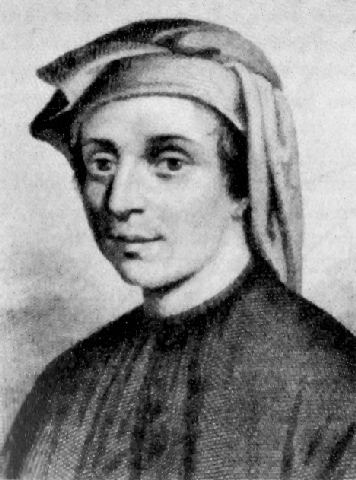
\includegraphics{images/fibonacci.jpg}

    {\tiny Source: https://en.wikipedia.org/wiki/ File:Fibonacci.jpg}
    
    \column{.7\textwidth}
    In 1202, Leonardo Bonacci (known as Fibonacci) asked the following
    question.

    \begin{tcolorbox}
      {\footnotesize ``[A]ssuming that: a newly born pair of rabbits,
        one male, one female, are put in a field; rabbits are able to
        mate at the age of one month so that at the end of its second
        month a female can produce another pair of rabbits; rabbits
        never die and a mating pair always produces one new pair (one
        male, one female) every month from the second month on.''

        ``The puzzle that Fibonacci posed was: how many pairs will
        there be in one year?''}
    \end{tcolorbox}
    
    {\tiny From https://en.wikipedia.org/wiki/Fibonacci\_number}
  \end{columns}
\end{frame}
